% The lattice {(a,b): b = 5a mod 13} (covolume 13) and the disk a^2+b^2 < 26 of area 26 pi > 4*13: it contains (2,-3), and 4+9 = 13.
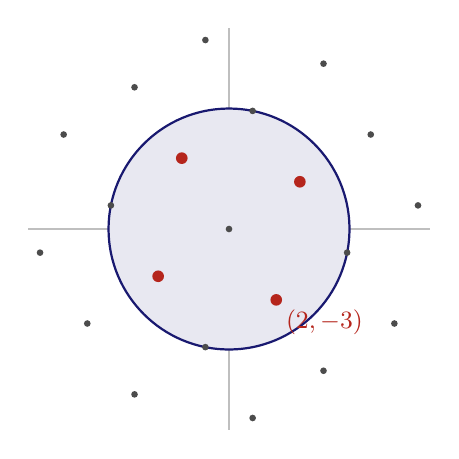
\begin{tikzpicture}[scale=0.3,font=\small]
\draw[black!25] (-8.5,0) -- (8.5,0) (0,-8.5) -- (0,8.5);
\draw[MidnightBlue,thick,fill=MidnightBlue!10] (0,0) circle (5.0990);
\fill[black!70] (-8.0000,-1.0000) circle (4pt);
\fill[black!70] (-7.0000,4.0000) circle (4pt);
\fill[black!70] (-6.0000,-4.0000) circle (4pt);
\fill[black!70] (-5.0000,1.0000) circle (4pt);
\fill[black!70] (-4.0000,-7.0000) circle (4pt);
\fill[black!70] (-4.0000,6.0000) circle (4pt);
\fill[black!70] (-3.0000,-2.0000) circle (4pt);
\fill[black!70] (-2.0000,3.0000) circle (4pt);
\fill[black!70] (-1.0000,-5.0000) circle (4pt);
\fill[black!70] (-1.0000,8.0000) circle (4pt);
\fill[black!70] (0.0000,0.0000) circle (4pt);
\fill[black!70] (1.0000,-8.0000) circle (4pt);
\fill[black!70] (1.0000,5.0000) circle (4pt);
\fill[black!70] (2.0000,-3.0000) circle (4pt);
\fill[black!70] (3.0000,2.0000) circle (4pt);
\fill[black!70] (4.0000,-6.0000) circle (4pt);
\fill[black!70] (4.0000,7.0000) circle (4pt);
\fill[black!70] (5.0000,-1.0000) circle (4pt);
\fill[black!70] (6.0000,4.0000) circle (4pt);
\fill[black!70] (7.0000,-4.0000) circle (4pt);
\fill[black!70] (8.0000,1.0000) circle (4pt);
\fill[BrickRed] (-3.0000,-2.0000) circle (7pt);
\fill[BrickRed] (-2.0000,3.0000) circle (7pt);
\fill[BrickRed] (2.0000,-3.0000) circle (7pt);
\fill[BrickRed] (3.0000,2.0000) circle (7pt);
\node[BrickRed,below right] at (2.0000,-3.0000) {$(2,-3)$};
\end{tikzpicture}
